\documentclass[border=15pt,multi=page,tikz]{standalone}
\usepackage{tikz}
\usepackage{amsmath}
\usetikzlibrary{arrows.meta,patterns,calc,angles,quotes}

\begin{document}

\begin{page}
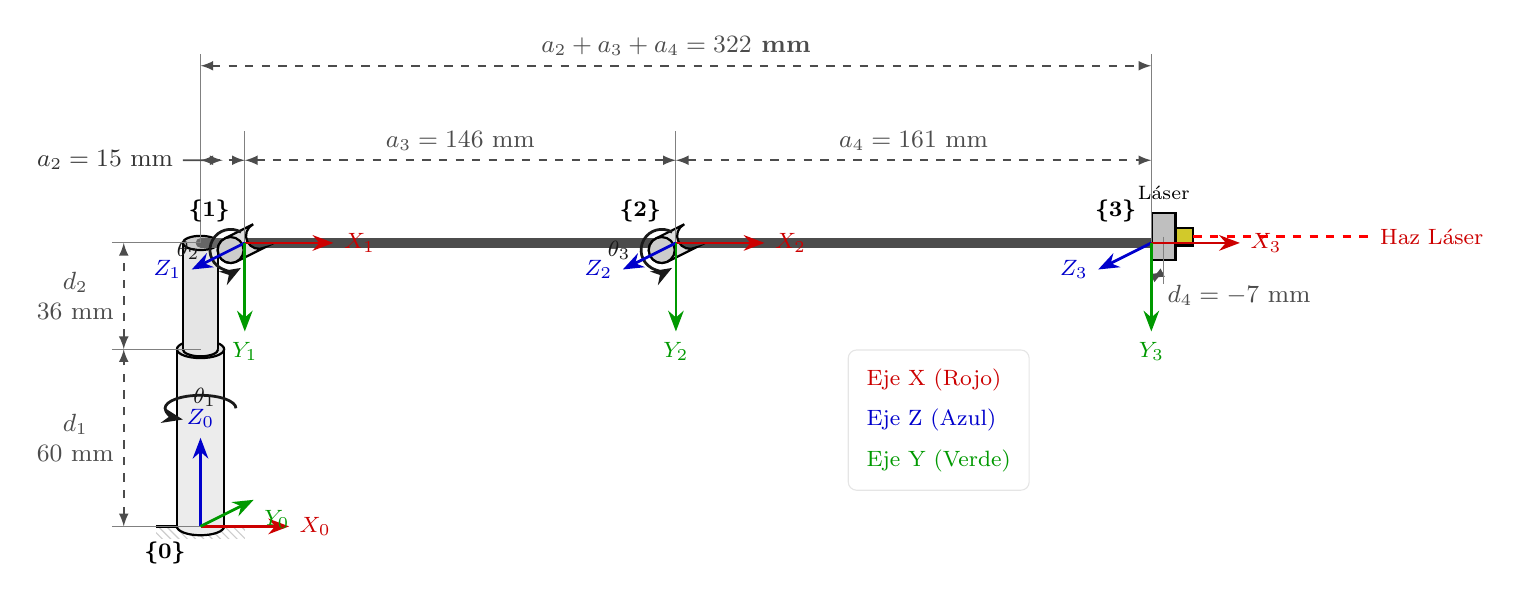
\begin{tikzpicture}[
    scale=0.75,
    >=Stealth,
    axis/.style={->,thick,line width=1.0pt},
    dim/.style={<->,>=latex,semithick,dashed,color=black!70},
    link/.style={line width=3.5pt,color=black!70,line cap=round},
    axisX/.style={axis,color=red!80!black},
    axisY/.style={axis,color=green!60!black},
    axisZ/.style={axis,color=blue!80!black}
]

    % Grid de ayuda (opcional, para depuración)
    %\draw[step=1cm,gray!15,very thin] (-2,-1) grid (22,15);

    % ==================== BASE FIJA (Ground hatching) ====================
    \fill[pattern=north west lines,pattern color=gray!40] (-0.75, -0.2) rectangle (0.75, 0);
    \draw[line width=1.2pt] (-0.75, 0) -- (0.75, 0);

    % ==================== PUNTOS CLAVE Y COORDENADAS ====================
    % Escala: 1 unit = 20 mm
    % Pedestal base (d1) = 60 mm = 3.0 units
    % Hombro desfasado (d2) = 36 mm = 1.8 units. Altura total base = 4.8 units
    % Offset hombro (a2) = 15 mm = 0.75 units
    % Longitud brazo (a3) = 146 mm = 7.3 units
    % Longitud antebrazo (a4) = 161 mm = 8.05 units
    
    \coordinate (O) at (0,0);
    \coordinate (BaseTop) at (0, 4.8);
    \coordinate (Shoulder) at (0.75, 4.8);
    \coordinate (Elbow) at (8.05, 4.8);
    \coordinate (Flange) at (16.1, 4.8);
    
    % Desfase transversal d4 = -7 mm = -0.35 units.
    % En nuestra proyección 3D, el eje X apunta en dirección (-0.6, -0.3).
    % Por lo tanto, un desfase d4 = -7 mm (sentido -X) se dibuja en dirección (0.6, 0.3):
    \coordinate (LaserTip) at ($(Flange) + 0.35*(0.6, 0.3)$);

    % ==================== DIBUJO DE LOS ESLABONES ====================
    % Eslabón fijo vertical (Base pedestal)
    \fill[gray!15] (-0.4, 0) rectangle (0.4, 3.0);
    \fill[gray!15] (0, 0) ellipse (0.4 and 0.15);
    \fill[gray!15] (0, 3.0) ellipse (0.4 and 0.15);
    \draw[line width=0.8pt] (-0.4, 0) -- (-0.4, 3.0);
    \draw[line width=0.8pt] (0.4, 0) -- (0.4, 3.0);
    \draw[line width=0.8pt] (0.4, 0) arc (0:-180:0.4 and 0.15);
    \draw[line width=0.8pt, fill=gray!25] (0, 3.0) ellipse (0.4 and 0.15);

    % Eslabón móvil vertical (Rotación base)
    \fill[gray!20] (-0.3, 3.0) rectangle (0.3, 4.8);
    \fill[gray!20] (0, 3.0) ellipse (0.3 and 0.12);
    \fill[gray!20] (0, 4.8) ellipse (0.3 and 0.12);
    \draw[line width=0.8pt] (-0.3, 3.0) -- (-0.3, 4.8);
    \draw[line width=0.8pt] (0.3, 3.0) -- (0.3, 4.8);
    \draw[line width=0.8pt] (0.3, 3.0) arc (0:-180:0.3 and 0.12);
    \draw[line width=0.8pt, fill=gray!40] (0, 4.8) ellipse (0.3 and 0.12);

    % Eslabón 1 (Base -> Hombro)
    \draw[link, color=black!60] (0, 4.8) -- (Shoulder);

    % Eslabón 2 (Hombro -> Codo)
    \draw[link] (Shoulder) -- (Elbow);

    % Eslabón 3 (Codo -> Brida)
    \draw[link] (Elbow) -- (Flange);

    % Acoplamiento al emisor láser (Transversal d4)
    \draw[line width=2.0pt, color=black!80] (Flange) -- (LaserTip);

    % ==================== JUNTAS CILÍNDRICAS (Estilo Craig/Spong) ====================
    % Junta 2: Hombro (Cilindro horizontal a lo largo del eje X)
    % Centro: (0.75, 4.8). Extremos a x=-0.4 y x=+0.4 (proyectados en 3D)
    % C1 (Atrás) = (0.75 + 0.24, 4.8 + 0.12) = (0.99, 4.92)
    % C2 (Adelante) = (0.75 - 0.24, 4.8 - 0.12) = (0.51, 4.68)
    \filldraw[fill=gray!25, draw=black, line width=0.8pt] 
      ($(0.99, 4.92) + (116.5:0.22)$) -- ($(0.51, 4.68) + (116.5:0.22)$) arc (116.5:296.5:0.22) -- ($(0.99, 4.92) + (296.5:0.22)$) arc (296.5:116.5:0.22);
    \draw[fill=gray!40, draw=black, line width=0.8pt] (0.51, 4.68) circle (0.22);

    % Junta 3: Codo (Cilindro horizontal paralelo al hombro)
    % Centro: (8.05, 4.8). Extremos a x=-0.4 y x=+0.4
    % C1 (Atrás) = (8.05 + 0.24, 4.8 + 0.12) = (8.29, 4.92)
    % C2 (Adelante) = (8.05 - 0.24, 4.8 - 0.12) = (7.81, 4.68)
    \filldraw[fill=gray!25, draw=black, line width=0.8pt] 
      ($(8.29, 4.92) + (116.5:0.22)$) -- ($(7.81, 4.68) + (116.5:0.22)$) arc (116.5:296.5:0.22) -- ($(8.29, 4.92) + (296.5:0.22)$) arc (296.5:116.5:0.22);
    \draw[fill=gray!40, draw=black, line width=0.8pt] (7.81, 4.68) circle (0.22);

    % Efector final: Diodo Láser en la punta
    \draw[fill=gray!50, draw=black, line width=0.8pt] ($(LaserTip)+(-0.2, -0.4)$) rectangle ($(LaserTip)+(0.2, 0.4)$);
    \draw[fill=yellow!80!black, draw=black, line width=0.8pt] ($(LaserTip)+(0.2, -0.15)$) -- ($(LaserTip)+(0.5, -0.15)$) -- ($(LaserTip)+(0.5, 0.15)$) -- ($(LaserTip)+(0.2, 0.15)$) -- cycle;
    \node[anchor=south, color=black, yshift=10pt, font=\scriptsize] at (LaserTip) {Láser};
    
    % Haz láser proyectado (rojo)
    \draw[red, dashed, line width=1.2pt] ($(LaserTip)+(0.5,0)$) -- ($(LaserTip)+(3.5,0)$);
    \node[anchor=west, color=red!80!black, font=\footnotesize] at ($(LaserTip)+(3.5,0)$) {Haz Láser};

    % ==================== ROTACIONES DE LAS JUNTAS ====================
    % Giro base theta1
    \draw[->, line width=1.0pt, color=black!90] (0.6, 2.0) arc (0:240:0.6 and 0.22) node[midway, right, font=\footnotesize] {$\theta_1$};
    
    % Giro hombro theta2 (alrededor de junta 2)
    \draw[->, line width=1.0pt, color=black!90] ($(0.51, 4.68) + (60:0.35)$) arc (60:300:0.35) node[midway, left, font=\footnotesize] {$\theta_2$};

    % Giro codo theta3 (alrededor de junta 3)
    \draw[->, line width=1.0pt, color=black!90] ($(7.81, 4.68) + (60:0.35)$) arc (60:300:0.35) node[midway, left, font=\footnotesize] {$\theta_3$};

    % ==================== COTAS Y MEDIDAS (Estilo CAD) ====================
    % Cotas d1 y d2 verticales
    \draw[dim] (-1.3, 0) -- (-1.3, 3.0) node[midway,left,align=center,font=\small] {$d_1$\\$60\text{ mm}$};
    \draw[dim] (-1.3, 3.0) -- (-1.3, 4.8) node[midway,left,align=center,font=\small] {$d_2$\\$36\text{ mm}$};
    \draw[gray,thin] (-1.5, 4.8) -- (0, 4.8);
    \draw[gray,thin] (-1.5, 3.0) -- (0, 3.0);
    \draw[gray,thin] (-1.5, 0) -- (O);

    % Cotas superiores
    \draw[gray,thin] (0, 4.8) -- (0, 6.7);
    \draw[gray,thin] (Shoulder) -- ($(Shoulder)+(0, 1.9)$);
    \draw[gray,thin] (Elbow) -- ($(Elbow)+(0, 1.9)$);
    \draw[gray,thin] (Flange) -- ($(Flange)+(0, 1.9)$);

    % Cota a2 (Offset base-hombro)
    \draw[dim] (0, 6.2) -- (0.75, 6.2);
    \node[anchor=east,font=\small,color=black!80] (a2label) at (-0.3, 6.2) {$a_2 = 15\text{ mm}$};
    \draw[->,>=latex,semithick,color=black!70] (a2label.east) -- (0.375, 6.2);

    % Cota a3 (Longitud Eslabón 2)
    \draw[dim] (0.75, 6.2) -- (8.05, 6.2) node[midway,above,font=\small] {$a_3 = 146\text{ mm}$};

    % Cota a4 (Longitud Eslabón 3)
    \draw[dim] (8.05, 6.2) -- (16.10, 6.2) node[midway,above,font=\small] {$a_4 = 161\text{ mm}$};

    % Cota total horizontal acumulada
    \draw[dim] (0, 7.8) -- (16.10, 7.8) node[midway,above,font=\small\bfseries] {$a_2 + a_3 + a_4 = 322\text{ mm}$};
    \draw[gray,thin] (0, 6.7) -- (0, 8.0);
    \draw[gray,thin] (Flange) -- ($(Flange)+(0, 3.2)$);

    % Cota del desfase transversal d4
    \draw[dim] (16.1, 4.2) -- ($(LaserTip) + (0, -0.6)$) node[midway, below right, font=\small] {$d_4 = -7\text{ mm}$};
    \draw[gray,thin] (16.1, 4.8) -- (16.1, 4.0);
    \draw[gray,thin] (LaserTip) -- ($(LaserTip) + (0, -0.8)$);

    % Leyenda de colores de ejes
    \matrix [draw=black!10,fill=white,fill opacity=0.9,text opacity=1.0,rounded corners=3pt,matrix anchor=center] at (12.5,1.8) {
      \node [red!80!black,anchor=west,font=\footnotesize] {Eje X (Rojo)}; \\
      \node [blue!80!black,anchor=west,font=\footnotesize] {Eje Z (Azul)}; \\
      \node [green!60!black,anchor=west,font=\footnotesize] {Eje Y (Verde)}; \\
    };

    % ==================== SISTEMAS DE REFERENCIA D-H ====================
    % Sistema 0 {0} - Base
    \draw[axisX] (O) -- (1.5,0) node[anchor=west,font=\footnotesize] {$X_0$};
    \draw[axisZ] (O) -- (0,1.5) node[anchor=south,font=\footnotesize] {$Z_0$};
    % Eje Y0 va hacia atrás en profundidad (-X de la pantalla, que es dirección 0.6, 0.3)
    \draw[axisY] (O) -- (0.9, 0.45) node[anchor=north west,font=\footnotesize] {$Y_0$};
    \node[anchor=north east,xshift=-2pt,yshift=-2pt,font=\footnotesize] at (O) {\textbf{\{0\}}};
 
    % Sistema 1 {1} - Hombro
    \begin{scope}[shift={(Shoulder)}]
        \draw[axisX] (0,0) -- (1.5,0) node[anchor=west,font=\footnotesize] {$X_1$};
        % Eje Z1 va hacia atrás (paralelo al eje de la junta revoluta horizontal, es decir, +X de pantalla: -0.6, -0.3)
        \draw[axisZ] (0,0) -- (-0.9,-0.45) node[anchor=east,font=\footnotesize] {$Z_1$};
        \draw[axisY] (0,0) -- (0,-1.5) node[anchor=north,font=\footnotesize] {$Y_1$};
        \node[anchor=south east,xshift=-2pt,yshift=4pt,font=\footnotesize] at (0,0) {\textbf{\{1\}}};
    \end{scope}

    % Sistema 2 {2} - Codo
    \begin{scope}[shift={(Elbow)}]
        \draw[axisX] (0,0) -- (1.5,0) node[anchor=west,font=\footnotesize] {$X_2$};
        \draw[axisZ] (0,0) -- (-0.9,-0.45) node[anchor=east,font=\footnotesize] {$Z_2$};
        \draw[axisY] (0,0) -- (0,-1.5) node[anchor=north,font=\footnotesize] {$Y_2$};
        \node[anchor=south east,xshift=-2pt,yshift=4pt,font=\footnotesize] at (0,0) {\textbf{\{2\}}};
    \end{scope}
 
    % Sistema 3 {3} - Efector Final
    \begin{scope}[shift={(Flange)}]
        \draw[axisX] (0,0) -- (1.5,0) node[anchor=west,font=\footnotesize] {$X_3$};
        \draw[axisZ] (0,0) -- (-0.9,-0.45) node[anchor=east,font=\footnotesize] {$Z_3$};
        \draw[axisY] (0,0) -- (0,-1.5) node[anchor=north,font=\footnotesize] {$Y_3$};
        \node[anchor=south east,xshift=-2pt,yshift=4pt,font=\footnotesize] at (0,0) {\textbf{\{3\}}};
    \end{scope}

\end{tikzpicture}
\end{page}

\begin{page}
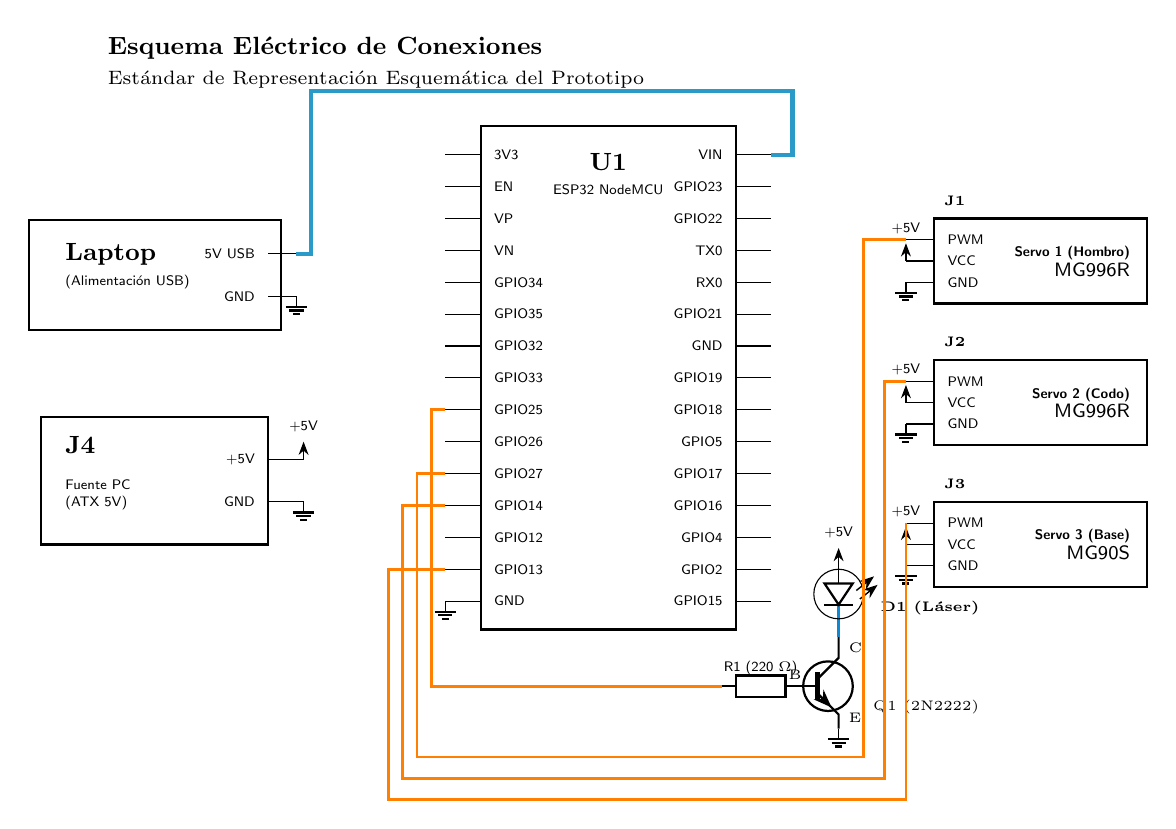
\begin{tikzpicture}[
    scale=0.9,
    >=Stealth,
    component/.style={rectangle,draw,thick,fill=white,draw=black,align=center},
    wire/.style={line width=1.0pt},
    labelStyle/.style={font=\footnotesize\sffamily}
]

    % Helper macros for GND and VCC symbols in TikZ
    \def\gnd(#1,#2){
        \draw (#1,#2) -- (#1,#2-0.15);
        \draw[thick] (#1-0.15,#2-0.15) -- (#1+0.15,#2-0.15);
        \draw[thick] (#1-0.1,#2-0.2) -- (#1+0.1,#2-0.2);
        \draw[thick] (#1-0.05,#2-0.25) -- (#1+0.05,#2-0.25);
    }
    \def\vcc(#1,#2){
        \draw[->, >=Stealth] (#1,#2) -- (#1,#2+0.25) node[anchor=south, font=\tiny\sffamily] {+5V};
    }

    % ==================== COMPONENTES ====================

    % Laptop (Fuente de alimentación USB)
    \node[component, minimum width=3.2cm, minimum height=1.4cm] (Laptop) at (-3.0, 5.0) {};
    \node[font=\bfseries\small, anchor=west] at (-4.4, 5.3) {Laptop};
    \node[font=\tiny\sffamily, anchor=west] at (-4.4, 4.9) {(Alimentación USB)};
    
    % Terminales de salida de Laptop
    \draw (-1.4, 5.3) -- (-1.0, 5.3);
    \node[anchor=east, font=\tiny\sffamily] at (-1.45, 5.3) {5V USB};
    \draw (-1.4, 4.7) -- (-1.0, 4.7);
    \node[anchor=east, font=\tiny\sffamily] at (-1.45, 4.7) {GND};
    \gnd(-1.0, 4.7)

    % Fuente de Alimentación de PC (ATX 5V - Conector J4)
    \draw[thick, fill=white] (-4.6, 1.2) rectangle (-1.4, 3.0);
    \node[font=\bfseries\small, anchor=west] at (-4.4, 2.6) {J4};
    \node[font=\tiny\sffamily, align=left, anchor=west] at (-4.4, 1.9) {Fuente PC\\(ATX 5V)};
    
    % Terminales de la fuente
    \draw (-1.4, 2.4) -- (-0.9, 2.4);
    \vcc(-0.9, 2.4)
    \node[font=\tiny\sffamily, anchor=east] at (-1.45, 2.4) {+5V};
    
    \draw (-1.4, 1.8) -- (-0.9, 1.8);
    \gnd(-0.9, 1.8)
    \node[font=\tiny\sffamily, anchor=east] at (-1.45, 1.8) {GND};

    % ESP32 DevKit NodeMCU (Símbolo Esquemático Completo U1)
    \draw[thick, fill=white] (1.6, 0.0) rectangle (5.2, 7.1);
    \node[font=\bfseries\small] at (3.4, 6.6) {U1};
    \node[font=\tiny\sffamily] at (3.4, 6.2) {ESP32 NodeMCU};

    % Pines del ESP32 - Izquierda (DIP-30 layout)
    \foreach \pinName [count=\i from 0] in {GND, GPIO13, GPIO12, GPIO14, GPIO27, GPIO26, GPIO25, GPIO33, GPIO32, GPIO35, GPIO34, VN, VP, EN, 3V3} {
        \pgfmathsetmacro{\y}{0.4 + 0.45 * \i}
        \draw (1.6, \y) -- (1.1, \y);
        \node[anchor=west, font=\tiny\sffamily] at (1.65, \y) {\pinName};
    }

    % Pines del ESP32 - Derecha (DIP-30 layout)
    \foreach \pinName [count=\i from 0] in {GPIO15, GPIO2, GPIO4, GPIO16, GPIO17, GPIO5, GPIO18, GPIO19, GND, GPIO21, RX0, TX0, GPIO22, GPIO23, VIN} {
        \pgfmathsetmacro{\y}{0.4 + 0.45 * \i}
        \draw (5.2, \y) -- (5.7, \y);
        \node[anchor=east, font=\tiny\sffamily] at (5.15, \y) {\pinName};
    }

    % Conector local a GND para el pin GND del ESP32 (izquierda abajo, y=0.4)
    \gnd(1.1, 0.4)

    % ==================== CONECTORES DE SERVOMOTORES ====================

    % Conector J1: Servo 1 (Hombro)
    \draw[thick, fill=white] (8.0, 4.6) rectangle (11.0, 5.8);
    \node[font=\bfseries\tiny, anchor=south west] at (8.0, 5.85) {J1};
    \node[font=\tiny\sffamily, align=right, anchor=east] at (10.9, 5.2) {\textbf{Servo 1 (Hombro)}\\ \scriptsize MG996R};
    % Pines del Conector J1
    \draw (8.0, 5.5) -- (7.6, 5.5); \node[anchor=west,font=\tiny\sffamily] at (8.05, 5.5) {PWM};
    \draw (8.0, 5.2) -- (7.6, 5.2); \node[anchor=west,font=\tiny\sffamily] at (8.05, 5.2) {VCC};
    \draw (8.0, 4.9) -- (7.6, 4.9); \node[anchor=west,font=\tiny\sffamily] at (8.05, 4.9) {GND};
    \vcc(7.6, 5.2)
    \gnd(7.6, 4.9)

    % Conector J2: Servo 2 (Codo)
    \draw[thick, fill=white] (8.0, 2.6) rectangle (11.0, 3.8);
    \node[font=\bfseries\tiny, anchor=south west] at (8.0, 3.85) {J2};
    \node[font=\tiny\sffamily, align=right, anchor=east] at (10.9, 3.2) {\textbf{Servo 2 (Codo)}\\ \scriptsize MG996R};
    % Pines del Conector J2
    \draw (8.0, 3.5) -- (7.6, 3.5); \node[anchor=west,font=\tiny\sffamily] at (8.05, 3.5) {PWM};
    \draw (8.0, 3.2) -- (7.6, 3.2); \node[anchor=west,font=\tiny\sffamily] at (8.05, 3.2) {VCC};
    \draw (8.0, 2.9) -- (7.6, 2.9); \node[anchor=west,font=\tiny\sffamily] at (8.05, 2.9) {GND};
    \vcc(7.6, 3.2)
    \gnd(7.6, 2.9)

    % Conector J3: Servo 3 (Base)
    \draw[thick, fill=white] (8.0, 0.6) rectangle (11.0, 1.8);
    \node[font=\bfseries\tiny, anchor=south west] at (8.0, 1.85) {J3};
    \node[font=\tiny\sffamily, align=right, anchor=east] at (10.9, 1.2) {\textbf{Servo 3 (Base)}\\ \scriptsize MG90S};
    % Pines del Conector J3
    \draw (8.0, 1.5) -- (7.6, 1.5); \node[anchor=west,font=\tiny\sffamily] at (8.05, 1.5) {PWM};
    \draw (8.0, 1.2) -- (7.6, 1.2); \node[anchor=west,font=\tiny\sffamily] at (8.05, 1.2) {VCC};
    \draw (8.0, 0.9) -- (7.6, 0.9); \node[anchor=west,font=\tiny\sffamily] at (8.05, 0.9) {GND};
    \vcc(7.6, 1.2)
    \gnd(7.6, 0.9)

    % ==================== CIRCUITO LÁSER CON NPN 2N2222 ====================

    % Resistencia de base 220 Ohm (R1)
    \draw[thick] (5.0, -0.8) -- (5.2, -0.8);
    \draw[thick, fill=white] (5.2, -0.95) rectangle (5.9, -0.65) node[midway, font=\tiny\sffamily, yshift=6.5pt] {R1 (220 $\Omega$)};
    \draw[thick] (5.9, -0.8) -- (6.2, -0.8);

    % Transistor NPN 2N2222 (Q1)
    \draw[thick] (6.5, -0.8) circle (0.35);
    \draw[line width=1.8pt] (6.35, -1.0) -- (6.35, -0.6); % Base bar
    \draw[thick] (6.2, -0.8) -- (6.35, -0.8) node[anchor=east, font=\tiny, xshift=-2pt, yshift=4pt] {B};
    \draw[thick] (6.35, -0.7) -- (6.65, -0.4) -- (6.65, -0.1) node[anchor=west, font=\tiny, yshift=-4pt] {C};
    \draw[thick] (6.35, -0.9) -- (6.65, -1.2) -- (6.65, -1.4) node[anchor=west, font=\tiny, yshift=4pt] {E};
    \draw[thick, ->, >=Stealth] (6.35, -0.9) -- (6.55, -1.1); % Emitter arrow
    \gnd(6.65, -1.4)
    \node[font=\tiny, anchor=west] at (7.0, -1.1) {Q1 (2N2222)};

    % Diodo Láser (D1)
    \draw[wire, cyan!70!blue] (6.65, -0.1) -- (6.65, 0.35); % Conexión cátodo a colector
    \draw[thick, fill=white] (6.45, 0.65) -- (6.85, 0.65) -- (6.65, 0.35) -- cycle; % Triángulo
    \draw[thick] (6.45, 0.35) -- (6.85, 0.35); % Barra de cátodo
    \draw (6.65, 0.5) circle (0.35); % Círculo
    \draw[->, >=Stealth, line width=0.5pt] (6.9, 0.55) -- (7.15, 0.75); % Flecha luz 1
    \draw[->, >=Stealth, line width=0.5pt] (6.95, 0.43) -- (7.2, 0.63); % Flecha luz 2
    \node[font=\bfseries\tiny, anchor=west] at (7.1, 0.3) {D1 (Láser)};
    
    \draw (6.65, 0.65) -- (6.65, 0.9);
    \vcc(6.65, 0.9)

    % ==================== CABLEADO / CONEXIONES ====================

    % Cable USB (Laptop -> ESP32 VIN)
    \draw[wire,cyan!80!black,line width=1.5pt] (-1.0, 5.3) -- (-0.8, 5.3) -- (-0.8, 7.6) -- (6.0, 7.6) -- (6.0, 6.7) -- (5.7, 6.7);

    % Señales (GPIO -> PWM de Servos)
    % GPIO 27 (y=2.2, left side, x=1.1) -> PWM Servo 1 (7.6, 5.5)
    \draw[wire,orange] (1.1, 2.2) -- (0.7, 2.2) -- (0.7, -1.8) -- (7.0, -1.8) -- (7.0, 5.5) -- (7.6, 5.5);
    
    % GPIO 14 (y=1.75, left side, x=1.1) -> PWM Servo 2 (7.6, 3.5)
    \draw[wire,orange] (1.1, 1.75) -- (0.5, 1.75) -- (0.5, -2.1) -- (7.3, -2.1) -- (7.3, 3.5) -- (7.6, 3.5);
    
    % GPIO 13 (y=0.85, left side, x=1.1) -> PWM Servo 3 (7.6, 1.5)
    \draw[wire,orange] (1.1, 0.85) -- (0.3, 0.85) -- (0.3, -2.4) -- (7.6, -2.4) -- (7.6, 1.5);

    % GPIO 25 (y=3.1, left side, x=1.1) -> Transistor Base (Láser)
    \draw[wire,orange] (1.1, 3.1) -- (0.9, 3.1) -- (0.9, -0.8) -- (5.0, -0.8);

    % Título del Diagrama
    \node[anchor=north west,align=left,font=\small] at (-3.8, 8.5) {
        \textbf{Esquema Eléctrico de Conexiones} \\
        \scriptsize Estándar de Representación Esquemática del Prototipo
    };

\end{tikzpicture}
\end{page}

\end{document}
